\documentclass[11pt]{article}

\usepackage[a4paper,margin=1in]{geometry}
\usepackage[T1]{fontenc}
\usepackage{lmodern}
\usepackage{microtype}
\usepackage{amsmath,amssymb}
\usepackage{array}
\usepackage{booktabs}
\usepackage{longtable}
\usepackage{tabularx}
\usepackage{graphicx}
\usepackage{xcolor}
\usepackage{hyperref}
\usepackage{enumitem}
\usepackage{seqsplit}
\usepackage{tikz}
\usetikzlibrary{arrows.meta,positioning,shapes.geometric,fit,backgrounds}

\hypersetup{
  colorlinks=true,
  linkcolor=blue!55!black,
  citecolor=blue!55!black,
  urlcolor=blue!55!black
}

\definecolor{ppBlue}{RGB}{33,79,140}
\definecolor{ppGreen}{RGB}{30,120,90}
\definecolor{ppGold}{RGB}{172,122,35}
\definecolor{ppGray}{RGB}{245,247,250}
\definecolor{ppLine}{RGB}{90,100,115}

\newcommand{\code}[1]{\texttt{#1}}
\newcommand{\breakcode}[1]{\begingroup\ttfamily\small\seqsplit{#1}\endgroup}
\newcommand{\sui}{\textsc{Sui}}
\newcommand{\walrus}{\textsc{Walrus}}
\newcommand{\pprf}{\code{PPRF}}
\newcommand{\manifest}{\code{deployment manifest}}

\graphicspath{{./figs/}}

\title{\textbf{PaperProof Protocol Yellow Paper}\\
\large A Source-Derived Specification of the Sui-Native Artifact Protocol}
\author{PaperProof Labs\\
\href{mailto:paperproof.labs@gmail.com}{paperproof.labs@gmail.com}\\
\href{https://paperproof.site/}{https://paperproof.site/}\\
\href{https://github.com/PaperProofLabs}{https://github.com/PaperProofLabs}}
\date{Draft v0.2 \\ June 2026}

\begin{document}
\maketitle

\section*{Copyright and Use Notice}

Copyright \copyright{} 2026 PaperProof Labs. All rights reserved.

This yellow paper is published as a source-available protocol specification for
review, citation, education, auditing, SDK development, indexing, and integration
with the official PaperProof Protocol deployments. Permission is granted to read,
download, print, quote limited portions, cite, and use this document for the
purpose of understanding, evaluating, or integrating with PaperProof.

No permission is granted by this document to use the PaperProof name, PaperProof
Labs name, logos, trademarks, deployment identity, official manifests, or other
branding in a confusing or misleading manner. No permission is granted to claim
that an independent implementation, fork, derivative protocol, or compatible
system is the official PaperProof Protocol unless expressly authorized by
PaperProof Labs or by the applicable future governance process.

This document does not relicense the PaperProof smart contracts, SDKs, website,
logos, trademarks, or other project materials. The smart-contract source code
remains governed by its own license notices, including
\code{LicenseRef-PaperProof-Source-Available} where applicable. Implementers are
responsible for complying with those licenses and with applicable law.

This document describes protocol concepts, object relationships, event
semantics, and deployment expectations. It is not a patent license, trademark
license, endorsement, warranty, or grant of official status. PaperProof Labs
reserves all rights not expressly granted here.

\begin{abstract}
PaperProof is a Sui-native protocol for durable, verifiable, and community-governed digital artifacts. This yellow paper specifies the current contract-level protocol as implemented by the PaperProof mainnet packages. It describes the trust roots, deployment manifest, object inventory, artifact type registry, artifact series model, typed version records, Walrus content references, comments tree, likes book, fee manager, governance vault, proposals, voting, claims, events, validation rules, error codes, indexing rules, upgrade boundaries, and SDK-facing contracts.

This document is intentionally narrower than a whitepaper and stricter than an application guide. It does not claim that PaperProof proves truth, originality, academic quality, license compliance, or social value. It specifies what the protocol recognizes, what the contracts store, what events can be treated as canonical under the active deployment, and how third-party applications and indexers should avoid common integration errors.
\end{abstract}

\tableofcontents
\newpage

\section{Status and Scope}

This document is derived from the PaperProof Move source code and deployment documentation in the contract repository. The relevant source modules are:

\begin{itemize}[leftmargin=*]
  \item \code{paperproof\_publishing::publishing}
  \item \code{paperproof\_publishing::artifact\_types}
  \item \code{paperproof\_publishing::validation}
  \item \code{paperproof\_comments::comments}
  \item \code{paperproof\_governance::governance}
  \item \code{paperproof\_governance::governance\_voting}
  \item \code{paperproof\_prompt\_registry::prompt\_registry}
  \item \code{paperproof\_memory\_registry::memory\_registry}
\end{itemize}

The default network is mainnet. Network-specific package and object bindings are not hardcoded into the abstract protocol. They are resolved through deployment manifests. The current mainnet manifest is summarized in Appendix~\ref{app:mainnet}. Future testnet manifests should follow the same schema.

\subsection{Normative Language}

The words ``MUST'', ``MUST NOT'', ``SHOULD'', and ``MAY'' are used in their ordinary specification sense. A frontend, SDK, or indexer that ignores a MUST-level condition may show incorrect protocol state, accept non-canonical events, or build transactions that are expected to fail.

\subsection{What This Yellow Paper Specifies}

This yellow paper specifies:

\begin{itemize}[leftmargin=*]
  \item protocol objects and their relationships;
  \item built-in artifact type constants and typed version records;
  \item publication and add-version state transitions;
  \item comment tree, blob comment, like, and unlike semantics;
  \item fee collection and fee level semantics;
  \item governance proposal, voting, execution, expiration, and claim semantics;
  \item event interpretation and canonical indexing rules;
  \item validation limits and abort-code tables;
  \item deployment manifest and drift-check expectations;
  \item SDK-facing behavior that follows from contract semantics.
\end{itemize}

\subsection{What This Yellow Paper Does Not Specify}

This document does not define a social feed, recommendation algorithm, full-text search system, moderation policy, peer-review process, airdrop rule, ranking algorithm, or token valuation model. It also does not make the official frontend or SDKs the source of protocol truth. The contracts and active deployment manifest define protocol bindings; SDKs and frontends are reference integration layers.

\section{System Overview}

PaperProof separates large content from compact authoritative state. \walrus{} stores large blobs such as PDFs, datasets, software archives, long comments, and static frontend assets. \sui{} stores official protocol objects, typed commitments, object bindings, fees, governance state, and canonical events. The protocol identity of an artifact is not merely a content hash or storage URL. It is a series object under an official root, with typed versions, official comments tree, official likes book, and events accepted under the active deployment.

\begin{figure}[htbp]
\centering
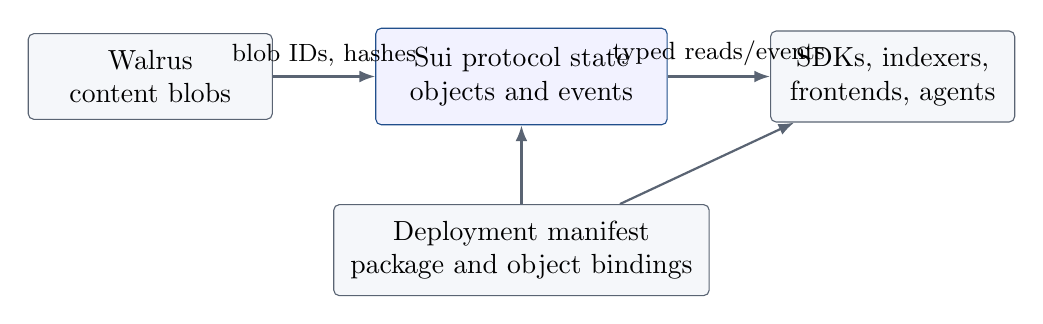
\begin{tikzpicture}[
  node distance=10mm,
  box/.style={draw=ppLine, rounded corners=2pt, fill=ppGray, inner sep=6pt, align=center, minimum width=31mm},
  core/.style={draw=ppBlue, rounded corners=2pt, fill=blue!5, inner sep=7pt, align=center, minimum width=37mm},
  arr/.style={-{Latex[length=2mm]}, thick, draw=ppLine}
]
\node[box] (content) {Walrus\\content blobs};
\node[core, right=13mm of content] (sui) {Sui protocol state\\objects and events};
\node[box, right=13mm of sui] (sdk) {SDKs, indexers,\\frontends, agents};
\node[box, below=10mm of sui] (manifestNode) {Deployment manifest\\package and object bindings};
\draw[arr] (content) -- node[above, font=\small]{blob IDs, hashes} (sui);
\draw[arr] (sui) -- node[above, font=\small]{typed reads/events} (sdk);
\draw[arr] (manifestNode) -- (sdk);
\draw[arr] (manifestNode) -- (sui);
\end{tikzpicture}
\caption{PaperProof separates content storage, protocol state, and integration surfaces.}
\label{fig:overview}
\end{figure}

\begin{figure}[htbp]
\centering
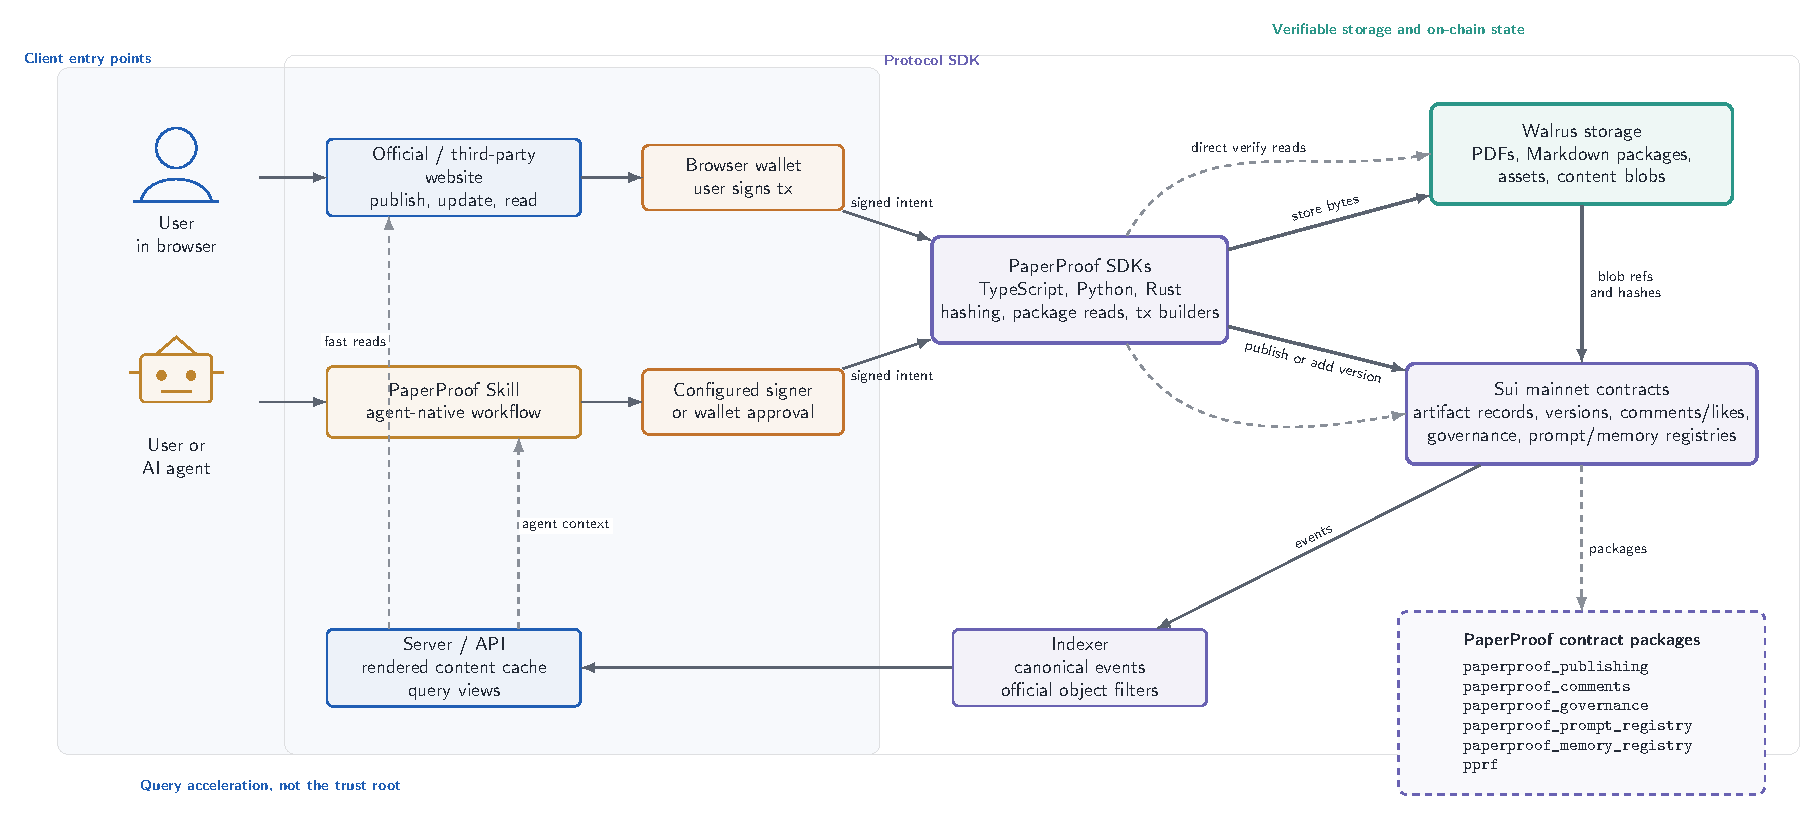
\includegraphics[width=0.7\textwidth]{application-architecture-flow.pdf}
\caption{Application-level architecture and flow. The official or third-party
website and the PaperProof Skill submit and query artifact workflows through
the same Sui mainnet contract packages, Walrus content layer, server-side
indexer, and SDK surfaces.}
\label{fig:application-architecture-flow}
\end{figure}

\section{Deployment Manifest}
\label{sec:manifest}

A PaperProof client MUST resolve network-specific package IDs, object IDs, coin types, and protocol version metadata from a deployment manifest. A deployment manifest is a JSON document with a schema version and a \code{deployment} object. It SHOULD also include package history so indexers can classify old events without treating them as current canonical events.

\subsection{Required Manifest Fields}

At minimum, a manifest MUST provide:

\begin{itemize}[leftmargin=*]
  \item network name, for example \code{mainnet} or future \code{testnet};
  \item protocol version label;
  \item package IDs for \code{pprf}, \code{publishing}, \code{comments}, and \code{governance};
  \item package IDs for optional official capability registries, including prompt and memory registries when enabled by an official app build;
  \item object IDs for the root, type registry, fee manager, governance vault, governance config, and \sui{} \code{Clock};
  \item object IDs for official shared capability registries where deployed;
  \item coin types for \pprf{}, \code{SUI}, and \code{WAL} where relevant;
  \item an update timestamp and minimum recommended SDK version.
\end{itemize}

\subsection{Drift Checks}

SDKs and indexers SHOULD fail closed when a manifest does not match chain state. A drift check SHOULD verify that:

\begin{itemize}[leftmargin=*]
  \item the root's governance vault, fee manager, and type registry IDs match the manifest;
  \item the governance vault's registry ID matches the official registry;
  \item the governance vault's governance config ID matches the manifest;
  \item the fee manager's registry ID matches the official registry;
  \item the comments trees and likes books accepted by the application are bound to official series objects;
  \item the prompt registry and memory registry, if used, bind to the same root ID and governance vault ID as the active manifest;
  \item event package IDs match the current package for current-state updates, while package history is used only for migration-aware historical views.
\end{itemize}

\section{Protocol Object Inventory}

Table~\ref{tab:object-inventory} lists the primary protocol objects. Getter functions exist for many fields; this paper lists semantic object roles rather than every read function.

\begin{longtable}{>{\raggedright\arraybackslash}p{0.25\textwidth}>{\raggedright\arraybackslash}p{0.65\textwidth}}
\caption{Primary protocol object inventory.}
\label{tab:object-inventory}\\
\toprule
\textbf{Object} & \textbf{Role} \\
\midrule
\endfirsthead
\toprule
\textbf{Object} & \textbf{Role} \\
\midrule
\endhead
\breakcode{PaperProofRoot} & Top-level trust anchor. Stores root version, paused flag, official governance vault ID, fee manager ID, type registry ID, comments tree factory capability, and governance action executor capability. \\
\breakcode{TypeRegistry} & Registry of supported artifact types. Stores registry version, registry ID, and a table from artifact type code to \code{TypeInfo}. \\
\breakcode{TypeInfo} & Per-type metadata: artifact type, type index object ID, enabled flag, schema version, minimum protocol version, creation timestamp, and update timestamp. \\
\breakcode{TypeIndex} & Per-type object used to support artifact code mapping and type-scoped discovery. It stores version, registry ID, and artifact type. \\
\breakcode{ArtifactSeries} & Stable identity of a continuing artifact. Stores type, code, owner, version IDs, current version, official comments tree, official likes book, status, UI status, metadata extensions, and timestamps. \\
\breakcode{CommonArtifactHeader} & Shared version header for all typed version records. Stores series ID, type, version number, previous version ID, author, content hash, Walrus references, content type, metadata extensions, status, and timestamp. \\
\breakcode{PreprintVersionRecord} & Typed version record for preprints. Adds title, abstract, authors, keywords, field, license, and page count. \\
\breakcode{BlogPostVersionRecord} & Typed version record for blog posts. Adds title, summary, tags, and language. \\
\breakcode{TechnicalReportVersionRecord} & Typed version record for technical reports. Adds title, abstract, authors, organization, report number, keywords, and license. \\
\breakcode{DatasetVersionRecord} & Typed version record for datasets. Adds title, description, format, file count, size in bytes, license, and keywords. \\
\breakcode{SoftwareReleaseVersionRecord} & Typed version record for software releases. Adds project name, version name, source hash, package hash, changelog, license, and repository URL. \\
\breakcode{GenericFileVersionRecord} & Typed version record for generic files. Adds title, description, filename, file size, and license. \\
\breakcode{CommentsTree} & Official comment space for a series. Stores target series, target artifact type, root comment, nodes table, owner, status, fee manager binding, max inline size, depth limit, and likes book ID. \\
\breakcode{CommentNode} & Single comment node. Stores parent, author, depth, content mode, inline content or blob references, children count, timestamps, and status. \\
\breakcode{LikesBook} & Official like state for a series. Stores comments tree ID, target series ID, target type, like count, and address-to-like table. \\
\breakcode{GovernanceVault} & Authority and treasury boundary. Stores governance authority, upgrade authority, active operator, pending operator transfer, fee recipient, direct authority mode, and related capability state. \\
\breakcode{FeeManager} & Official fee configuration. Stores registry ID and fee levels for comments and artifact types. \\
\breakcode{GovernanceConfig} & Proposal system configuration. Stores total supply, proposer threshold, duration, next proposal ID, pause state, active proposal ID, proposal ID mapping, and enabled actions. \\
\breakcode{Proposal} & Governance proposal object. Stores proposal type, action type, title, description, payload fields, votes, locked balances, epoch window, status, execution flag, and vote records. \\
\breakcode{PromptRegistry} & Official route-to-prompt registry for app prompts. Stores root binding, governance vault binding, and prompt registrations keyed by app ID and route ID. Updates require the active governance operator. \\
\breakcode{PromptRegistration} & Copyable prompt binding record. Stores app ID, route ID, prompt artifact series ID, optional pinned version ID, latest-version policy, schema version, update epoch, and updater. \\
\breakcode{MemoryRegistry} & Official Copilot memory capability registry. Stores root binding, governance vault binding, provider policies, and active memory entry IDs by wallet owner and app ID. \\
\breakcode{ProviderPolicy} & Memory provider policy. Stores provider name, enabled flag, accepted schema-version range, update epoch, and updater. \\
\breakcode{MemoryEntry} & Per-wallet, per-app memory capability object. Stores owner, app ID, memory ID, provider, MemWal account ID, namespace root, descriptor artifact code, descriptor series/version policy, schema version, availability, owner-enabled state, owner-deleted tombstone, and timestamps. \\
\bottomrule
\end{longtable}

\section{Artifact Types}

Artifact types are protocol-recognized constants. They are not arbitrary labels. Adding a new protocol-recognized type is a contract and SDK change followed by governance activation.

\begin{table}[htbp]
\centering
\caption{Built-in artifact types.}
\label{tab:artifact-types}
\begin{tabular}{cll}
\toprule
\textbf{Value} & \textbf{Name} & \textbf{Primary typed record} \\
\midrule
1 & \code{preprint} & \code{PreprintVersionRecord} \\
2 & \code{blog\_post} & \code{BlogPostVersionRecord} \\
3 & \code{technical\_report} & \code{TechnicalReportVersionRecord} \\
4 & \code{dataset} & \code{DatasetVersionRecord} \\
5 & \code{software\_release} & \code{SoftwareReleaseVersionRecord} \\
6 & \code{generic\_file} & \code{GenericFileVersionRecord} \\
\bottomrule
\end{tabular}
\end{table}

The artifact code function constructs a human-readable code:

\[
\code{PaperProof-\{type\}-\{epoch6\}-\{series\_id\_hex12\}}
\]

The artifact code is useful for display and search, but the authoritative identity remains the series object ID plus official root and registry binding.

\section{Artifact Series and Version Records}

\subsection{Series Identity}

\code{ArtifactSeries} is the protocol identity of a continuing work. A series MUST have exactly one artifact type and one artifact code. A series MAY have many versions up to \code{MAX\_VERSIONS\_PER\_SERIES = 168}. The current implementation stores version IDs in a vector and tracks the current version number and current version object ID.

Series status values are:

\begin{table}[htbp]
\centering
\caption{Series status values.}
\begin{tabular}{cl}
\toprule
\textbf{Value} & \textbf{Meaning} \\
\midrule
0 & active \\
1 & locked \\
2 & hidden \\
\bottomrule
\end{tabular}
\end{table}

Only active series are intended to receive normal new versions. Hidden status is a protocol field that official applications may interpret as non-display state. Status changes emit \code{ArtifactStatusChangedEvent}.

\subsection{Common Version Header}

Every typed version record contains \code{CommonArtifactHeader}. This header is the shared commitment layer. It binds the version to:

\begin{itemize}[leftmargin=*]
  \item series ID;
  \item artifact type;
  \item version number;
  \item previous version ID if present;
  \item author address;
  \item content hash;
  \item Walrus blob ID;
  \item Walrus blob object ID;
  \item content type;
  \item bounded metadata extensions;
  \item version status;
  \item chain timestamp in milliseconds.
\end{itemize}

The current version status constant is \code{VERSION\_STATUS\_VALID = 0}. Version records are shared objects once created and are not mutated by later version additions.

\subsection{Metadata Extensions}

Series and version metadata extensions are vectors of \code{MetadataAttribute}. Limits are:

\begin{table}[htbp]
\centering
\caption{Metadata extension limits.}
\begin{tabular}{lr}
\toprule
\textbf{Limit} & \textbf{Value} \\
\midrule
\code{MAX\_METADATA\_ATTRIBUTES} & 4 \\
\code{MAX\_METADATA\_KEY\_BYTES} & 64 \\
\code{MAX\_METADATA\_VALUE\_BYTES} & 511 \\
\bottomrule
\end{tabular}
\end{table}

Keys MUST be non-empty and unique within the vector. Metadata extensions are display and indexing aids; they MUST NOT be used as the sole authority for core protocol semantics.

\section{Publication and Version State Transitions}

\subsection{Publication}

Publication functions are type-specific:

\begin{itemize}[leftmargin=*]
  \item \code{publish\_preprint}
  \item \code{publish\_blog\_post}
  \item \code{publish\_technical\_report}
  \item \code{publish\_dataset}
  \item \code{publish\_software\_release}
  \item \code{publish\_generic\_file}
\end{itemize}

Each publication call MUST provide the official root, type registry, governance vault, fee manager, type-specific metadata, common content fields, optional series and version metadata extensions, optional \code{SUI} payment, \sui{} \code{Clock}, and transaction context.

Publication performs the following logical steps:

\begin{enumerate}[leftmargin=*]
  \item validate type-specific metadata and common content fields;
  \item verify root, registry, vault, and fee manager bindings;
  \item verify the protocol is not paused;
  \item verify the artifact type is supported and enabled;
  \item collect the configured artifact fee, if any;
  \item create an \code{ArtifactSeries};
  \item create a typed version record with version number 1;
  \item create the official comments tree and likes book;
  \item share the series, comments tree, likes book, and typed version record;
  \item emit \code{ArtifactPublishedEvent} and related creation events.
\end{enumerate}

\subsection{Adding Versions}

Add-version functions are also type-specific:

\begin{itemize}[leftmargin=*]
  \item \code{add\_preprint\_version}
  \item \code{add\_blog\_post\_version}
  \item \code{add\_technical\_report\_version}
  \item \code{add\_dataset\_version}
  \item \code{add\_software\_release\_version}
  \item \code{add\_generic\_file\_version}
\end{itemize}

An add-version transaction MUST be authorized by the current series owner, MUST match the series artifact type, MUST keep the series within the maximum version count, MUST use official root/registry/vault/fee manager bindings, and MUST produce a typed version record for the same artifact type. It emits \code{ArtifactVersionAddedEvent}.

\subsection{Ownership Transfer}

\code{transfer\_artifact\_owner} changes the owner of a series. The caller MUST be the current series owner. The new owner MUST be nonzero. The implementation also updates the official comments tree owner boundary so that moderation authority follows artifact ownership.

\section{Walrus Content References}

PaperProof does not store large content bytes in \sui{} objects. Instead, version records store content references:

\begin{itemize}[leftmargin=*]
  \item \code{content\_hash}: application-selected content digest string;
  \item \code{walrus\_blob\_id}: Walrus blob identifier;
  \item \code{walrus\_blob\_object\_id}: Walrus blob object identifier;
  \item \code{content\_type}: media type or application content type string.
\end{itemize}

The contract validates that these fields are non-empty and within bounded lengths. SDKs SHOULD verify content locally before publication when possible. The protocol records the commitment; it does not download or validate blob bytes inside Move.

\section{Comments Tree and Likes Book}

\subsection{Official Binding}

Every published artifact series receives an official \code{CommentsTree} and \code{LikesBook}. A frontend or indexer MUST NOT accept an arbitrary comments tree as official only because it has the expected Move type. It MUST verify that the series object stores the tree ID and likes book ID, and that the tree/book fields bind to the same registry, series, and artifact type.

\subsection{Comment Tree Status and Comment Status}

\begin{table}[htbp]
\centering
\caption{Comment tree and comment status values.}
\begin{tabular}{lll}
\toprule
\textbf{Domain} & \textbf{Value} & \textbf{Meaning} \\
\midrule
Tree & 0 & open \\
Tree & 1 & locked \\
Tree & 2 & archived \\
Comment & 0 & active \\
Comment & 1 & hidden \\
Comment & 2 & deleted \\
\bottomrule
\end{tabular}
\end{table}

Only open trees accept new comments. A parent comment MUST exist and MUST be active. The root comment has ID 0 and cannot be mutated as an ordinary user comment.

An application MAY use tree status to create non-commentable official surfaces.
For example, Docs articles can be published as ordinary artifact series while
their official comments tree is set to \code{locked} or \code{archived}. The
frontend SHOULD hide comment controls for such surfaces, but the protocol reason
new comments fail is the tree status check.

\subsection{On-Chain and Blob Comments}

Comment content modes are:

\begin{table}[htbp]
\centering
\caption{Comment content modes.}
\begin{tabular}{cl}
\toprule
\textbf{Value} & \textbf{Meaning} \\
\midrule
1 & inline on-chain content \\
2 & blob-backed content \\
\bottomrule
\end{tabular}
\end{table}

Inline comments MUST be non-empty and no larger than the tree's configured
maximum inline-comment byte limit, whose default is 512 bytes. Blob comments
MUST include non-empty blob ID and blob digest and MAY include a content
preview. Blob comment limits are:

\begin{table}[htbp]
\centering
\caption{Blob comment limits.}
\begin{tabular}{lr}
\toprule
\textbf{Limit} & \textbf{Value} \\
\midrule
\code{MAX\_BLOB\_ID\_BYTES} & 128 \\
\code{MAX\_BLOB\_DIGEST\_BYTES} & 128 \\
\code{MAX\_CONTENT\_PREVIEW\_BYTES} & 256 \\
\code{DEFAULT\_MAX\_COMMENT\_DEPTH} & 64 \\
\bottomrule
\end{tabular}
\end{table}

\subsection{Comment Moderation}

The tree owner may set tree status and comment status. A comment author may delete their own comment, but cannot restore hidden comments or modify the root comment. Deleted comments are final for status purposes. Status changes emit \code{TreeStatusChangedEvent} or \code{CommentStatusChangedEvent}.

\subsection{Likes}

\code{like\_paper} and \code{unlike\_paper} operate on the official \code{LikesBook}. The caller MUST provide a \pprf{} coin proof whose value is at least \code{MIN\_PPRF\_FOR\_LIKE}. A like is proof of holding, not a burn or stake. The likes book prevents duplicate likes by the same address and emits \code{PaperLikedEvent} or \code{PaperUnlikedEvent}.

\section{Protocol-Native Prompt Registry}

The prompt registry maps official application routes to versioned PaperProof
prompt artifacts. Prompt bytes are not stored in the registry. They are stored
as ordinary \code{generic\_file} artifacts whose version records commit to
Walrus references. The registry only selects which artifact series and version
policy an official app route should use.

\subsection{Prompt Registration Key}

A prompt registration is keyed by \code{app\_id + ":" + route\_id}. In the
official app, examples include \code{paperproof-app:copilot/global} and
\code{paperproof-app:copilot/memory}. The registry stores:

\begin{itemize}[leftmargin=*]
  \item \code{app\_id} and \code{route\_id};
  \item \code{series\_id} of the prompt artifact;
  \item optional \code{pinned\_version\_id};
  \item \code{use\_latest}, which selects the current version of the series when true;
  \item \code{schema\_version};
  \item update epoch and updater address.
\end{itemize}

\subsection{Prompt Governance Boundary}

\code{create\_registry} and \code{register\_prompt} MUST be called by the active
operator of the root-bound governance vault. The registry MUST bind to the same
root ID and governance vault ID expected by the active deployment manifest.
This is intentionally lighter than proposal-based automatic execution: it gives
official operators a governed capability boundary without requiring every prompt
update to be a full token vote.

Clients MUST resolve prompt content in two steps. First, read the official
prompt registration. Second, read the referenced PaperProof artifact
series/version through normal artifact rules. If \code{use\_latest} is false,
\code{pinned\_version\_id} MUST be present. If chain resolution, Walrus fetch, or
manifest drift checks fail, an app MAY fall back to bundled prompts, but it MUST
not claim those bundled prompts are the current chain-selected prompt.

\section{Copilot Memory Registry}

The memory registry is a governed discovery and availability layer for
wallet-linked Copilot memory. It does not store private memory bodies. Memory
bodies are handled by an external provider such as MemWal, which may in turn use
Walrus storage. PaperProof stores only metadata needed for official discovery,
version policy, and availability checks.

\subsection{Provider Policy}

Before a provider is considered usable, the registry MUST contain a
\code{ProviderPolicy}. A policy records provider name, enabled flag, minimum and
maximum accepted schema versions, update epoch, and updater. Setting provider
policy requires the active governance operator.

\subsection{Memory Entry State}

Each \code{MemoryEntry} is a shared object. The official app model is at most
one active entry per wallet owner and app ID. Deleted entries are tombstoned,
not physically erased, and the active-entry mapping is released so the owner can
create a new entry later.

\begin{table}[htbp]
\centering
\caption{Memory entry usability flags.}
\begin{tabularx}{\textwidth}{p{0.22\textwidth}X}
\toprule
\textbf{Field} & \textbf{Meaning} \\
\midrule
\code{available} & Operator/governance availability flag. If false, the official Copilot MUST NOT use the entry. \\
\code{owner\_enabled} & User-controlled enablement flag for the chain entry. \\
\code{owner\_deleted} & Tombstone flag. Deleted entries are not usable and do not block later registration. \\
\code{use\_latest} & Version policy for the descriptor artifact. If false, a pinned version ID is required. \\
\bottomrule
\end{tabularx}
\end{table}

A memory entry is usable only when all of the following hold: it belongs to the
official registry, \code{available} is true, \code{owner\_enabled} is true,
\code{owner\_deleted} is false, the provider policy exists, the provider policy
is enabled, and the entry schema version is within the provider policy range.

\subsection{Memory Operations}

The create-entry function creates a shared entry and records its ID in the
owner/app active-entry table. The call MUST reject creation if an active entry
already exists for the same owner and app ID. The update-pointer function lets
the owner update the provider account pointer and namespace root. The
disable-entry function lets the owner set \code{owner\_enabled} to false. The
delete-entry function releases the active-entry mapping, sets
\code{owner\_enabled} to false, sets \code{owner\_deleted} to true, sets
\code{available} to false, and records a deletion epoch. It does not delete
external MemWal or Walrus data.

\code{set\_memory\_availability} and \code{set\_memory\_version\_policy} require
the active governance operator and the official registry/vault binding. They
let the official app disable a specific memory capability or change the
descriptor series/version policy used to explain the memory schema.

\section{Fee Model}

\code{FeeManager} stores fee levels rather than arbitrary per-call fee values. The current fee level constants are:

\begin{table}[htbp]
\centering
\caption{Fee level constants.}
\begin{tabular}{cl}
\toprule
\textbf{Value} & \textbf{Name} \\
\midrule
0 & free \\
1 & micro \\
2 & low \\
3 & standard \\
4 & high \\
\bottomrule
\end{tabular}
\end{table}

Comments use fee key \code{FEE\_KEY\_COMMENTS = 0}. Artifact publishing and versioning use artifact-type fee levels. Fees are collected through the official governance vault and fee manager. A fake fee manager with the same field names MUST NOT be accepted by clients.

\section{Governance}

\subsection{Governance Vault}

\code{GovernanceVault} is the authority boundary for governance and operational roles. It stores:

\begin{itemize}[leftmargin=*]
  \item governance config ID;
  \item governance authority;
  \item upgrade authority;
  \item active operator and operator epoch;
  \item pending operator transfer state;
  \item fee recipient;
  \item direct authority mode;
  \item permanent direct-authority-disable flag.
\end{itemize}

Direct authority modes are:

\begin{table}[htbp]
\centering
\caption{Direct authority modes.}
\begin{tabular}{cl}
\toprule
\textbf{Value} & \textbf{Meaning} \\
\midrule
0 & full \\
1 & emergency \\
2 & read-only \\
3 & disabled \\
\bottomrule
\end{tabular}
\end{table}

Permanent disablement is one-way. Once direct authority is permanently disabled, the protocol cannot return to a stronger direct-authority mode.

\subsection{Governance Config and Proposals}

\code{GovernanceConfig} stores proposal parameters, action enablement, active proposal tracking, and proposal ID mapping. \code{Proposal} stores proposal metadata, payload, vote totals, locked \pprf{} balances, epoch window, status, and per-address vote records.

Proposal types are:

\begin{table}[htbp]
\centering
\caption{Proposal types.}
\begin{tabular}{cl}
\toprule
\textbf{Value} & \textbf{Meaning} \\
\midrule
1 & executable \\
2 & signal \\
\bottomrule
\end{tabular}
\end{table}

Proposal status values are:

\begin{table}[htbp]
\centering
\caption{Proposal status values.}
\begin{tabular}{cl}
\toprule
\textbf{Value} & \textbf{Meaning} \\
\midrule
1 & active \\
2 & passed \\
3 & rejected \\
4 & executed \\
5 & expired \\
\bottomrule
\end{tabular}
\end{table}

\subsection{Governance Action Types}

\begin{longtable}{cl}
\caption{Governance action type constants.}
\label{tab:governance-actions}\\
\toprule
\textbf{Value} & \textbf{Action} \\
\midrule
\endfirsthead
\toprule
\textbf{Value} & \textbf{Action} \\
\midrule
\endhead
2 & set comments fee level \\
3 & set fee recipient \\
4 & nominate operator \\
5 & set proposal creation paused \\
6 & set proposer threshold \\
7 & set upgrade authority \\
8 & set proposal duration epochs \\
9 & set artifact type enabled \\
10 & set artifact fee level \\
11 & activate artifact type \\
12 & set governance action enabled \\
13 & set direct authority mode \\
14 & cancel operator transfer \\
15 & set governance authority \\
101 & signal replace operator \\
102 & signal feature direction \\
103 & signal policy position \\
\bottomrule
\end{longtable}

\subsection{Voting and Claims}

Proposal creation requires a proposer stake of \pprf{} at least equal to the configured proposer threshold. The proposer stake is counted as a yes vote and locked in the proposal. Additional voters call \code{vote\_yes} or \code{vote\_no} with \pprf{} coins. Minimum vote stake is \code{100\_000\_000\_000} base units, documented in code as 100 \pprf{}.

After voting ends, \code{finalize\_proposal} determines whether the proposal passed or failed. \code{resolve\_proposal\_early} may finalize early only when the outcome is determinable. After a proposal leaves active status, voters can call \code{claim\_locked\_tokens} to recover locked funds. A voter can claim only once because the vote record is removed during claim.

\subsection{Execution}

Executable proposals can be executed after passing and before execution expiry. The general \code{execute\_proposal} path handles actions that mutate the governance vault or config directly, such as fee recipient, operator nomination, pause flag, proposer threshold, upgrade authority, proposal duration, governance action enablement, direct authority mode, and governance authority.

Some actions are intentionally consumed through a \code{GovernanceActionTicket} and then applied by target modules. This pattern is used for artifact type enabled, artifact fee level, artifact type activation, and comments fee level. The ticket prevents a generic proposal from becoming an unrestricted capability.

\section{Events}

Events are evidence for off-chain systems, but they are not self-authenticating. A canonical event MUST come from the active package and MUST match the official root, registry, vault, fee manager, series, comments tree, or likes book binding expected for the event type.

\subsection{Publishing Events}

Publishing emits:

\begin{itemize}[leftmargin=*]
  \item \code{PaperProofRootCreatedEvent}
  \item \code{TypeRegistryCreatedEvent}
  \item \code{TypeIndexCreatedEvent}
  \item \code{ArtifactPublishedEvent}
  \item \code{ArtifactVersionAddedEvent}
  \item \code{ArtifactStatusChangedEvent}
  \item \code{ArtifactSeriesMetadataUpdatedEvent}
  \item \code{ArtifactTypeStatusChangedEvent}
  \item \code{ProtocolPausedChangedEvent}
\end{itemize}

\subsection{Comment and Like Events}

Comment and like events are:

\begin{itemize}[leftmargin=*]
  \item \code{TreeCreatedEvent}
  \item \code{CommentAddedEvent}
  \item \code{TreeStatusChangedEvent}
  \item \code{CommentStatusChangedEvent}
  \item \code{TreeOwnerTransferredEvent}
  \item \code{CommentsTreeMigratedEvent}
  \item \code{PaperLikedEvent}
  \item \code{PaperUnlikedEvent}
\end{itemize}

\subsection{Governance Events}

Governance emits:

\begin{itemize}[leftmargin=*]
  \item creation events: \breakcode{GovernanceVaultCreatedEvent}, \breakcode{FeeManagerCreatedEvent}, and \breakcode{GovernanceConfigCreatedEvent};
  \item proposal events: \breakcode{ProposalCreatedEvent}, \breakcode{VoteCastEvent}, \breakcode{ProposalFinalizedEvent}, \breakcode{ProposalExecutedEvent}, \breakcode{ProposalExpiredEvent}, and \breakcode{VoteClaimedEvent};
  \item parameter events: \breakcode{ProposalCreationPausedChangedEvent}, \breakcode{ProposerThresholdChangedEvent}, \breakcode{ProposalDurationChangedEvent}, and \breakcode{GovernanceActionStatusChangedEvent};
  \item authority events: \breakcode{OperatorNominatedEvent}, \breakcode{OperatorTransferAcceptedEvent}, \breakcode{OperatorTransferCancelledEvent}, \breakcode{GovernanceAuthorityChangedEvent}, \breakcode{UpgradeAuthorityChangedEvent}, and \breakcode{DirectAuthorityModeChangedEvent};
  \item fee and upgrade events: \breakcode{FeeCollectedEvent}, \breakcode{CommentsFeeLevelChangedEvent}, \breakcode{ArtifactFeeLevelChangedEvent}, \breakcode{ManagedUpgradeCapRegisteredEvent}, \breakcode{ManagedUpgradeAuthorizedEvent}, and \breakcode{ManagedUpgradeCommittedEvent}.
\end{itemize}

\subsection{Prompt Registry Events}

Prompt registry events are:

\begin{itemize}[leftmargin=*]
  \item \code{PromptRegistryCreatedEvent}
  \item \code{PromptRegisteredEvent}
\end{itemize}

\subsection{Memory Registry Events}

Memory registry events are:

\begin{itemize}[leftmargin=*]
  \item \code{MemoryRegistryCreatedEvent}
  \item \code{ProviderPolicySetEvent}
  \item \code{MemoryEntryCreatedEvent}
  \item \code{MemoryEntryPointerUpdatedEvent}
  \item \code{MemoryEntryDeletedEvent}
  \item \code{MemoryEntryAvailabilitySetEvent}
  \item \code{MemoryEntryVersionPolicySetEvent}
\end{itemize}

\section{Canonical Indexing Rules}

Indexers are part of the protocol integration surface. They MUST distinguish accepted events from rejected events.

\subsection{Canonical Acceptance}

An event SHOULD update canonical domain state only if:

\begin{enumerate}[leftmargin=*]
  \item its package ID matches the current package ID for the relevant module in the active manifest;
  \item the event's registry/root/vault/fee manager fields match the active manifest or an official object reachable from it;
  \item for artifact events, the series object belongs to the official publishing path and its artifact type is supported;
  \item for comment events, the tree ID matches the series's official comments tree ID;
  \item for like events, the likes book ID matches the series's official likes book ID;
  \item for governance events, the proposal belongs to the official governance config and registry;
  \item for prompt events, the prompt registry ID, root ID, and governance vault ID match the active manifest;
  \item for memory events, the memory registry ID, root ID, governance vault ID, entry registry ID, and active-entry mapping match the active manifest and object state.
\end{enumerate}

Events from historical packages MAY be retained in a non-current historical table, but frontends MUST NOT report current state as complete if they only query an old package or omit active package filters.

\subsection{Derived API Views}

Indexer APIs MAY expose derived views such as artifact summaries, type lists,
search results, lookup responses, official content caches, and wallet activity
views. These views are integration products, not new protocol truth. A derived
view SHOULD include enough source material for clients to explain how it was
constructed: artifact code, series ID, latest version ID, content hash, Walrus
blob references, timestamp, accepted package, and cache or refresh time where
relevant.

An indexer that exposes derived views MUST continue to apply the canonical
acceptance rules above. It MUST NOT promote stale package events, rejected
events, failed Walrus reads, or application display policy into protocol facts.
When a derived view is incomplete because of provider failure, cache warmup,
object hydration failure, or Walrus unavailability, it SHOULD report degraded
status rather than silently returning an empty state.

\subsection{Empty State vs Failed Query}

Applications MUST distinguish:

\begin{itemize}[leftmargin=*]
  \item no canonical events found;
  \item provider failed;
  \item provider page limit reached;
  \item drift check failed;
  \item old-package events exist but current-package events do not;
  \item object read succeeded but dynamic child content failed.
\end{itemize}

Showing ``no votes'', ``no comments'', or ``no artifacts'' when the provider failed is a protocol integration bug.

\subsection{Protocol Facts vs Interface Policy}

An official or third-party interface MAY hide, delist, de-rank, label, refuse
to preview, or decline to index an artifact, comment, link, or Walrus
reference. Such interface policy MUST NOT be represented as deletion of
underlying protocol facts. Sui records, third-party indexer records, and
decentralized-storage content may remain retrievable even when one interface
does not display them.

Likewise, a visible artifact MUST NOT be interpreted as endorsed, reviewed, or
certified by the interface operator. PaperProof establishes typed commitments
and official object relationships. It does not establish content truth, legal
compliance, academic merit, safety, or social approval.

Independent applications, indexers, wallets, dashboards, agents, and direct
chain clients MAY reconstruct protocol views from official objects and
canonical events. They MAY apply their own display and moderation policies, but
they SHOULD clearly distinguish those application-layer choices from
contract-level status and storage availability.

\section{Validation Rules}

Table~\ref{tab:validation-limits} summarizes the public validation limits in the publishing and comments modules.

\begin{longtable}{lr}
\caption{Validation limits.}
\label{tab:validation-limits}\\
\toprule
\textbf{Limit} & \textbf{Value} \\
\midrule
\endfirsthead
\toprule
\textbf{Limit} & \textbf{Value} \\
\midrule
\endhead
\code{MAX\_VERSIONS\_PER\_SERIES} & 168 \\
\code{MAX\_METADATA\_ATTRIBUTES} & 4 \\
\code{MAX\_METADATA\_KEY\_BYTES} & 64 \\
\code{MAX\_METADATA\_VALUE\_BYTES} & 511 \\
\code{MAX\_KEYWORDS} & 10 \\
\code{MAX\_AUTHORS} & 20 \\
\code{MAX\_TAGS} & 20 \\
\code{MAX\_TITLE\_BYTES} & 256 \\
\code{MAX\_LONG\_TEXT\_BYTES} & 4096 \\
\code{MAX\_MEDIUM\_TEXT\_BYTES} & 1024 \\
\code{MAX\_SHORT\_TEXT\_BYTES} & 256 \\
\code{MAX\_VECTOR\_ITEM\_BYTES} & 128 \\
\code{MAX\_CONTENT\_HASH\_BYTES} & 128 \\
\code{MAX\_WALRUS\_BLOB\_ID\_BYTES} & 128 \\
\code{MAX\_WALRUS\_BLOB\_OBJECT\_ID\_BYTES} & 128 \\
\code{MAX\_CONTENT\_TYPE\_BYTES} & 64 \\
\code{DEFAULT\_MAX\_ONCHAIN\_COMMENT\_BYTES} & 512 \\
\code{DEFAULT\_MAX\_COMMENT\_DEPTH} & 64 \\
\bottomrule
\end{longtable}

\section{SDK-Facing Contracts}

SDKs are not protocol truth, but they SHOULD encode the following rules:

\begin{itemize}[leftmargin=*]
  \item load deployment manifests without hardcoding only mainnet;
  \item default to mainnet unless the user selects another network;
  \item validate Sui addresses, object IDs, package IDs, artifact types, content fields, metadata attributes, and string lengths before building transactions;
  \item expose build-only, dry-run, dev-inspect, sign-and-execute, and typed-result helpers where the underlying platform supports them;
  \item return typed IDs extracted from transaction results, including series ID, version ID, comments tree ID, likes book ID, comment ID, proposal ID, and digest;
  \item expose prompt registry builders and prompt resolution helpers that support latest and pinned version policies;
  \item expose memory registry builders for creating, deleting, disabling, and governing memory entries without treating private memory bodies as chain data;
  \item expose query providers and watch APIs that apply canonical filters;
  \item preserve cause chains in errors and avoid treating provider failure as empty protocol state;
  \item expose Walrus content helper functions for publish, read, verify, extend, and owned-blob transfer while preserving Walrus ownership and shared-blob semantics.
\end{itemize}

For static frontend deployments, browser access to third-party model endpoints,
Walrus gateways, and memory relayers depends on ordinary web network policy such
as CORS. This is not a Move protocol rule. A local development server may proxy
MemWal relayer calls for demos, while a production static site requires a
browser-compatible relayer or accepts graceful degradation of memory save/recall
without breaking ordinary artifact, prompt, and governance reads.

SDKs SHOULD also support transaction composition where it preserves contract
semantics. Compatible Move calls MAY be grouped into a Sui Programmable
Transaction Block so a user signs one coherent artifact action. Integrators
MUST still respect storage-provider phase boundaries: for example, Walrus
reserve and certify operations may require distinct stages even when later
certification, publication, add-version, or registry-update calls can be
composed.

\subsection{Reference Indexer API Expectations}

The reference indexer MAY provide server-assisted endpoints for the official
application, including Explore summary, type-scoped item lists, search, lookup,
official Docs/Blog/Forum content, and compatibility routes for older clients.
Those endpoints SHOULD be understood as SDK-facing integration surfaces. They
MUST preserve the same canonical filtering rules as persistent indexer tables.

A reference API MAY expose endpoints such as health, JSON metrics, Prometheus
metrics, artifact exploration, artifact search, artifact detail, versions,
comments, activity, governance proposals, wallet-owned artifacts, wallet votes,
analytics summaries, and deterministic airdrop snapshots. These endpoints MUST
be documented as derived read APIs. They MUST NOT be described as additional
Move entrypoints or as replacements for Sui object state, Walrus content
references, deployment manifests, or canonical event acceptance.

Official public content caches SHOULD be keyed by the official manifest entry,
series ID, selected version ID, content hash, and Walrus blob reference. A cache
hit MAY return verified markdown, package metadata, or rendered-safe content
without repeating the full Walrus fetch path. A cache miss or event-driven
refresh MUST re-check the chain object or normalized latest version and verify
the content hash before presenting content as verified. For Docs/Blog/Forum
entries, event-driven refresh is preferred; periodic reconciliation is only a
fallback for missed events, manifest drift, service restart, or provider
transient failure.

\section{Upgrade and Compatibility}

PaperProof is upgradeable during its early protocol phase. Package IDs may change. Object IDs for root, registry, vault, and fee manager may remain stable across some upgrades but MUST NOT be assumed without a manifest and drift check.

If only package bindings change and entry signatures/event schemas remain compatible, a manifest update may be enough for many clients. If entry signatures, object layouts, event schemas, or semantic rules change, SDKs and indexers SHOULD publish new versions. Indexers SHOULD store package history so they can explain historical events without mixing them into current canonical state.

\section{Security Boundaries}

PaperProof security depends on explicit object binding. The following rules are critical:

\begin{itemize}[leftmargin=*]
  \item The official root is the trust entry point.
  \item A matching Move type is insufficient to prove an object is official.
  \item Comments and likes are official only through the series-bound tree and book.
  \item Governance events are official only through the active governance config and vault.
  \item Fee settings are official only through the root-bound fee manager.
  \item Prompt registrations are official only through the manifest-bound prompt registry and referenced PaperProof artifact series.
  \item Memory entries are official only through the manifest-bound memory registry and usable only when provider, availability, owner, and deletion checks pass.
  \item Large content remains outside Move; on-chain records commit to references and hashes, not to bytes.
  \item Private Copilot memory bodies are not stored in PaperProof Move objects.
  \item PPRF likes and votes are participation signals; they do not prove merit or truth.
  \item AI agents and frontends may explain and prepare transactions, but wallets or signers remain the authority boundary.
\end{itemize}

\section{Implementation Evidence and Verification Surfaces}

This yellow paper is normative only where it describes contract and integration
rules. The following figures are included as implementation evidence for the
current official deployment and developer workflow. They are not themselves
protocol authority.

\begin{figure}[htbp]
  \centering
  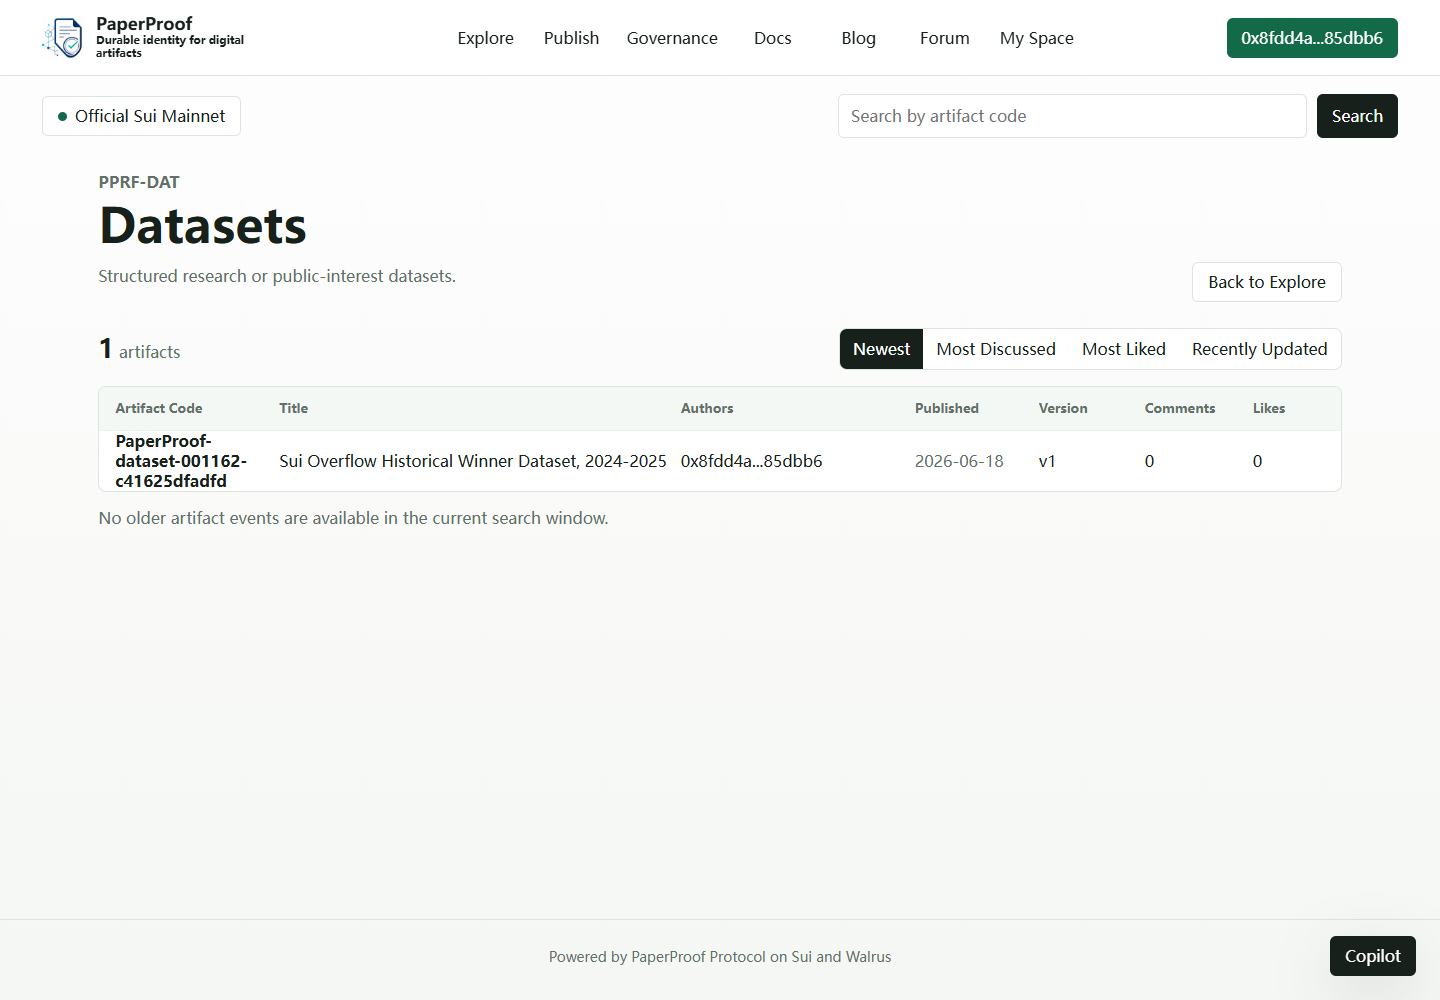
\includegraphics[width=0.7\textwidth]{datasets-type-list.png}
  \caption{A reference application view derived from canonical artifact events
  and indexer APIs. Derived views must remain explainable in terms of protocol
  objects and accepted events.}
  \label{fig:yellow-datasets-view}
\end{figure}

\begin{figure}[htbp]
  \centering
  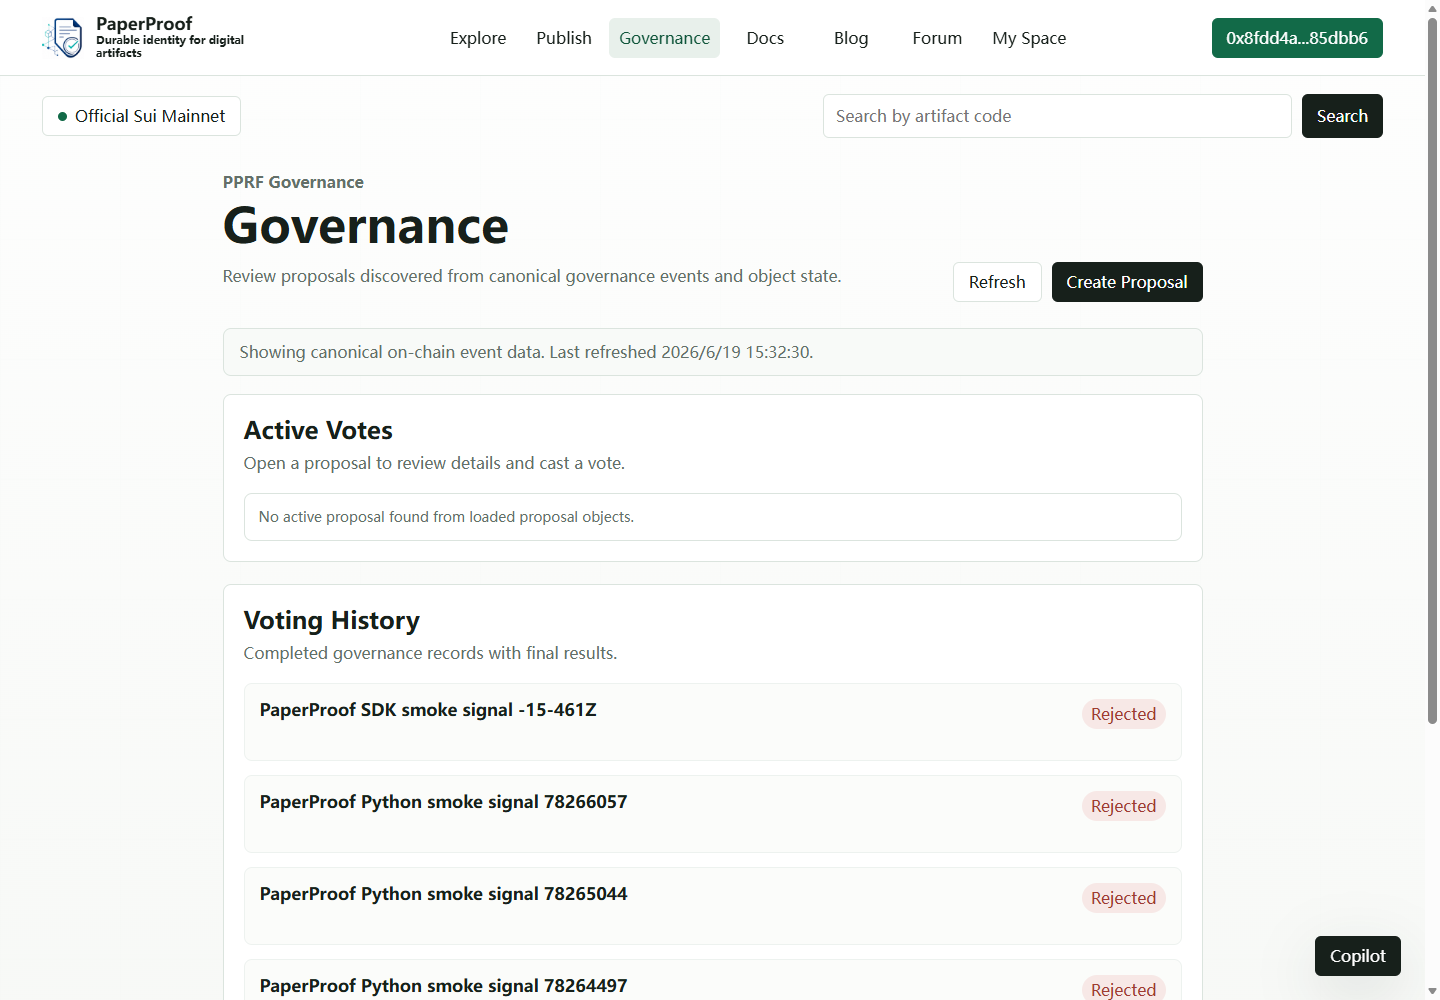
\includegraphics[width=0.7\textwidth]{governance-page.png}
  \caption{Governance views expose active proposals and voting records, but
  client display policy must remain distinct from contract-level proposal and
  voting state.}
  \label{fig:yellow-governance-view}
\end{figure}

\begin{figure}[htbp]
  \centering
  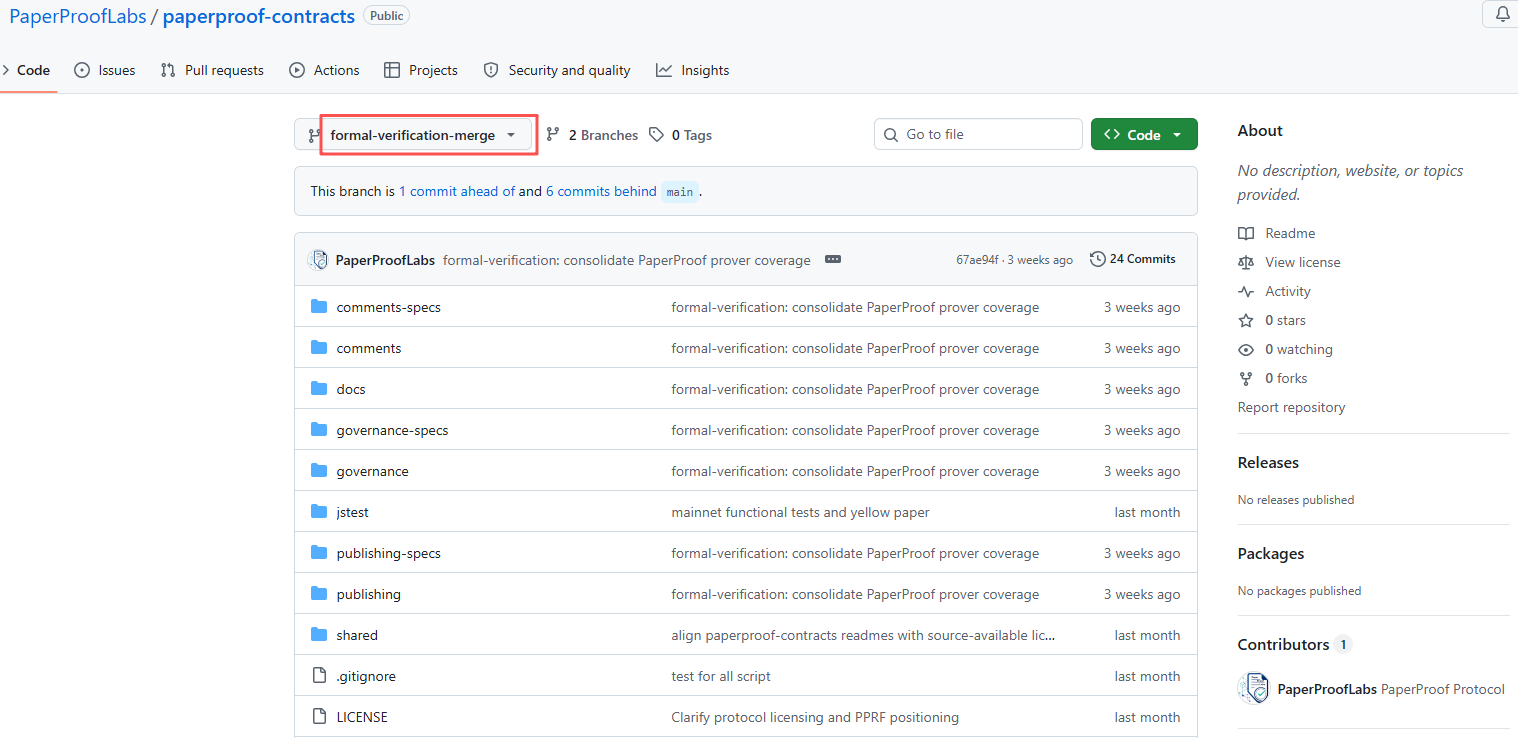
\includegraphics[width=0.7\textwidth]{formal-verification-branch.png}
  \caption{The contracts repository maintains a formal-verification-oriented
  branch/view alongside implementation sources. Formal artifacts are evidence
  and review aids; active deployment identity still comes from the manifest and
  on-chain object bindings.}
  \label{fig:yellow-formal-verification}
\end{figure}

\appendix

\section{Mainnet Deployment Snapshot}
\label{app:mainnet}

The current mainnet manifest records:

\begin{longtable}{>{\raggedright\arraybackslash}p{0.25\textwidth}>{\raggedright\arraybackslash}p{0.65\textwidth}}
\caption{Mainnet package and object bindings.}\\
\toprule
\textbf{Name} & \textbf{Value} \\
\midrule
\endfirsthead
\toprule
\textbf{Name} & \textbf{Value} \\
\midrule
\endhead
\code{network} & \breakcode{mainnet} \\
\code{protocolVersion} & \breakcode{publishing-v3-governance-v2-comments-v2} \\
\code{pprf package} & \breakcode{0x5d2ec9829a9e116de7c2008281a90b96690beb2252af120ad05a25fe13fae0da} \\
\code{publishing package} & \breakcode{0xc9a75e4514db2a37df6f95b4e2b329c065ac6089953bd2c1c0a0c389835bd3d8} \\
\code{comments package} & \breakcode{0xaef346fc40bf20af62f4bbbc1608ba2272e80e4ba3d716634026baa589e9aeba} \\
\code{governance package} & \breakcode{0xc1ced3b8ae5281eeeb8cdb5527978e294c54f14a7fd8d65e7e9502d4ffffb87e} \\
\code{prompt registry package} & \breakcode{0x10b9c6e90a896dc3244d047e32724d80de0dc697b5ea12c5fdd8925131ed4c59} \\
\code{memory registry package} & \breakcode{0xbe9527ee927c4a6dcb91d5503758cd731d311813cd70d93914f2bf58a36db3d1} \\
\code{root} & \breakcode{0x7dc6c78b276825499a2204b060394e80b81196eb1f77d2036b503a2cca15dd78} \\
\code{typeRegistry} & \breakcode{0x966ffa24d0a96b34267b62c628f39c830afc9de25438b6502835fa8a3815d6b5} \\
\code{feeManager} & \breakcode{0x7bb8360ea1fa50f923628c929b8726b00eb8968c6a678acde71f97ae146e9249} \\
\code{governanceVault} & \breakcode{0x0df35aa53ef37f8ca8f6a6280d743effa6e0bfc613c5c6c0a78318ad4a38f875} \\
\code{governanceConfig} & \breakcode{0x7ed018db6b2cd7c32692a1c33543fb90d9c36add1226f93cbeb2a8fb10955dfa} \\
\code{promptRegistry} & \breakcode{0x14ec45eb83bb1b0eb22c7e885c7c71ea05b1e22dd05e3e1107dcef528600b0da} \\
\code{memoryRegistry} & \breakcode{0x9a5beeb6610b33c06771c4152c039314784437e802e200afd2ce80fb88bdf9e2} \\
\code{clock} & \breakcode{0x6} \\
\code{PPRF coin type} & \breakcode{0x5d2ec9829a9e116de7c2008281a90b96690beb2252af120ad05a25fe13fae0da::pprf::PPRF} \\
\bottomrule
\end{longtable}

\section{Abort Code Summary}

\subsection{Publishing Abort Codes}

\begin{longtable}{lr}
\toprule
\textbf{Name} & \textbf{Code} \\
\midrule
\endfirsthead
\toprule
\textbf{Name} & \textbf{Code} \\
\midrule
\endhead
\code{E\_PAUSED} & 1 \\
\code{E\_UNSUPPORTED\_ROOT\_VERSION} & 2 \\
\code{E\_UNSUPPORTED\_REGISTRY\_VERSION} & 3 \\
\code{E\_UNSUPPORTED\_SERIES\_VERSION} & 4 \\
\code{E\_INVALID\_ARTIFACT\_TYPE} & 5 \\
\code{E\_ARTIFACT\_TYPE\_DISABLED} & 6 \\
\code{E\_INVALID\_INDEX} & 7 \\
\code{E\_INVALID\_GOVERNANCE\_VAULT} & 8 \\
\code{E\_INVALID\_FEE\_MANAGER} & 9 \\
\code{E\_NOT\_OWNER} & 21 \\
\code{E\_INVALID\_STATUS} & 22 \\
\code{E\_INVALID\_COMMENTS\_TREE} & 23 \\
\code{E\_INVALID\_GOVERNANCE\_ACTION} & 24 \\
\code{E\_TOO\_MANY\_VERSIONS} & 25 \\
\code{E\_TOO\_MANY\_METADATA\_ATTRIBUTES} & 26 \\
\code{E\_EMPTY\_METADATA\_KEY} & 27 \\
\code{E\_METADATA\_TEXT\_TOO\_LONG} & 28 \\
\code{E\_DUPLICATE\_METADATA\_KEY} & 29 \\
\bottomrule
\end{longtable}

\subsection{Validation Abort Codes}

\begin{longtable}{lr}
\toprule
\textbf{Name} & \textbf{Code} \\
\midrule
\endfirsthead
\toprule
\textbf{Name} & \textbf{Code} \\
\midrule
\endhead
\code{E\_EMPTY\_CONTENT\_HASH} & 10 \\
\code{E\_EMPTY\_BLOB\_ID} & 11 \\
\code{E\_EMPTY\_BLOB\_OBJECT\_ID} & 12 \\
\code{E\_EMPTY\_CONTENT\_TYPE} & 13 \\
\code{E\_EMPTY\_TITLE} & 14 \\
\code{E\_EMPTY\_AUTHOR\_LIST} & 17 \\
\code{E\_TOO\_MANY\_KEYWORDS} & 18 \\
\code{E\_TOO\_MANY\_AUTHORS} & 19 \\
\code{E\_TOO\_MANY\_TAGS} & 20 \\
\code{E\_TEXT\_TOO\_LONG} & 21 \\
\code{E\_EMPTY\_TEXT} & 22 \\
\code{E\_EMPTY\_VECTOR\_ITEM} & 23 \\
\bottomrule
\end{longtable}

\subsection{Comments Abort Codes}

\begin{longtable}{lr}
\toprule
\textbf{Name} & \textbf{Code} \\
\midrule
\endfirsthead
\toprule
\textbf{Name} & \textbf{Code} \\
\midrule
\endhead
\code{E\_EMPTY\_TARGET\_KEY} & 1 \\
\code{E\_TREE\_NOT\_OPEN} & 2 \\
\code{E\_PARENT\_NOT\_FOUND} & 3 \\
\code{E\_EMPTY\_ONCHAIN\_CONTENT} & 4 \\
\code{E\_ONCHAIN\_CONTENT\_TOO\_LARGE} & 5 \\
\code{E\_EMPTY\_BLOB\_ID} & 6 \\
\code{E\_EMPTY\_BLOB\_DIGEST} & 7 \\
\code{E\_NOT\_TREE\_OWNER} & 8 \\
\code{E\_INVALID\_TREE\_STATUS} & 9 \\
\code{E\_INVALID\_COMMENT\_STATUS} & 10 \\
\code{E\_COMMENT\_NOT\_FOUND} & 11 \\
\code{E\_NOT\_COMMENT\_OWNER\_OR\_TREE\_OWNER} & 12 \\
\code{E\_COMMENT\_DEPTH\_LIMIT} & 13 \\
\code{E\_INVALID\_GOVERNANCE\_VAULT} & 14 \\
\code{E\_INVALID\_NEW\_OWNER} & 15 \\
\code{E\_INSUFFICIENT\_PPRF\_LIKE\_BALANCE} & 16 \\
\code{E\_ALREADY\_LIKED} & 17 \\
\code{E\_NOT\_LIKED} & 18 \\
\code{E\_UNSUPPORTED\_TREE\_VERSION} & 19 \\
\code{E\_PARENT\_NOT\_ACTIVE} & 20 \\
\code{E\_BLOB\_ID\_TOO\_LONG} & 21 \\
\code{E\_BLOB\_DIGEST\_TOO\_LONG} & 22 \\
\code{E\_CONTENT\_PREVIEW\_TOO\_LONG} & 23 \\
\code{E\_INVALID\_TREE\_FACTORY\_CAP} & 24 \\
\code{E\_ROOT\_COMMENT\_IMMUTABLE} & 25 \\
\code{E\_DELETED\_COMMENT\_FINAL} & 26 \\
\bottomrule
\end{longtable}

\subsection{Prompt Registry Abort Codes}

\begin{longtable}{lr}
\toprule
\textbf{Name} & \textbf{Code} \\
\midrule
\endfirsthead
\toprule
\textbf{Name} & \textbf{Code} \\
\midrule
\endhead
\code{E\_INVALID\_GOVERNANCE} & 1 \\
\code{E\_EMPTY\_APP\_ID} & 2 \\
\code{E\_EMPTY\_ROUTE\_ID} & 3 \\
\code{E\_INVALID\_VERSION\_POLICY} & 4 \\
\code{E\_PROMPT\_NOT\_FOUND} & 5 \\
\code{E\_ZERO\_ROOT} & 6 \\
\code{E\_TEXT\_TOO\_LONG} & 7 \\
\bottomrule
\end{longtable}

\subsection{Memory Registry Abort Codes}

\begin{longtable}{lr}
\toprule
\textbf{Name} & \textbf{Code} \\
\midrule
\endfirsthead
\toprule
\textbf{Name} & \textbf{Code} \\
\midrule
\endhead
\code{E\_INVALID\_GOVERNANCE} & 1 \\
\code{E\_EMPTY\_APP\_ID} & 2 \\
\code{E\_EMPTY\_PROVIDER} & 3 \\
\code{E\_EMPTY\_NAMESPACE\_ROOT} & 4 \\
\code{E\_TEXT\_TOO\_LONG} & 5 \\
\code{E\_ZERO\_ACCOUNT} & 6 \\
\code{E\_EMPTY\_MEMORY\_ID} & 7 \\
\code{E\_EMPTY\_ARTIFACT\_CODE} & 8 \\
\code{E\_INVALID\_VERSION\_POLICY} & 9 \\
\code{E\_NOT\_OWNER} & 10 \\
\code{E\_ZERO\_SERIES} & 11 \\
\code{E\_PROVIDER\_NOT\_FOUND} & 12 \\
\code{E\_ACTIVE\_ENTRY\_EXISTS} & 13 \\
\bottomrule
\end{longtable}

\subsection{Governance Voting Abort Codes}

\begin{longtable}{lr}
\toprule
\textbf{Name} & \textbf{Code} \\
\midrule
\endfirsthead
\toprule
\textbf{Name} & \textbf{Code} \\
\midrule
\endhead
\code{E\_ZERO\_TOTAL\_SUPPLY} & 1 \\
\code{E\_PROPOSAL\_CREATION\_PAUSED} & 2 \\
\code{E\_INVALID\_PROPOSAL\_TYPE} & 3 \\
\code{E\_INVALID\_ACTION\_TYPE} & 4 \\
\code{E\_PROPOSAL\_NOT\_ACTIVE} & 5 \\
\code{E\_ALREADY\_VOTED} & 6 \\
\code{E\_VOTING\_NOT\_ENDED} & 7 \\
\code{E\_PROPOSAL\_ALREADY\_FINALIZED} & 8 \\
\code{E\_PROPOSAL\_NOT\_PASSED} & 9 \\
\code{E\_PROPOSAL\_NOT\_EXECUTABLE} & 10 \\
\code{E\_PROPOSAL\_ALREADY\_EXECUTED} & 11 \\
\code{E\_INVALID\_BOOLEAN\_PAYLOAD} & 12 \\
\code{E\_INVALID\_VAULT\_REGISTRY} & 13 \\
\code{E\_VOTING\_ALREADY\_ENDED} & 14 \\
\code{E\_EXECUTABLE\_ACTION\_NOT\_ALLOWED} & 15 \\
\code{E\_SIGNAL\_ACTION\_NOT\_ALLOWED} & 16 \\
\code{E\_ACTIVE\_PROPOSAL\_EXISTS} & 17 \\
\code{E\_PROPOSAL\_NOT\_FINALIZED} & 18 \\
\code{E\_NO\_VOTE\_TO\_CLAIM} & 19 \\
\code{E\_VOTING\_POWER\_BELOW\_MINIMUM} & 20 \\
\code{E\_PROPOSER\_STAKE\_BELOW\_THRESHOLD} & 21 \\
\code{E\_INVALID\_PROPOSER\_THRESHOLD} & 22 \\
\code{E\_UNSUPPORTED\_CONFIG\_VERSION} & 23 \\
\code{E\_UNSUPPORTED\_PROPOSAL\_VERSION} & 24 \\
\code{E\_INVALID\_PROPOSAL\_DURATION\_EPOCHS} & 25 \\
\code{E\_PROPOSAL\_EXECUTION\_NOT\_EXPIRED} & 26 \\
\code{E\_PROPOSAL\_OUTCOME\_NOT\_YET\_DETERMINABLE} & 27 \\
\code{E\_ACTION\_NOT\_ENABLED} & 28 \\
\code{E\_INVALID\_ACTION\_ENABLE\_TARGET} & 29 \\
\code{E\_NOT\_GOVERNANCE\_CONFIG\_INITIALIZER} & 30 \\
\code{E\_INVALID\_PROPOSAL\_CONFIG\_BINDING} & 31 \\
\code{E\_EMPTY\_PROPOSAL\_TITLE} & 32 \\
\code{E\_PROPOSAL\_TEXT\_TOO\_LONG} & 33 \\
\bottomrule
\end{longtable}

\section{References}

\begin{itemize}[leftmargin=*]
  \item PaperProof contracts repository, Move source modules listed in Section 1.
  \item PaperProof deployment manifest, \code{docs/deployments/mainnet.json}.
  \item Sui documentation: \url{https://docs.sui.io/}.
  \item Walrus documentation: \url{https://docs.wal.app/}.
\end{itemize}

\end{document}
